\documentclass[10pt]{article}
\usepackage[utf8]{inputenc}

\newcommand{\documenttitle}{CSC311 Final Project}
\newcommand{\documentauthor}{Ian Huang, Benjamin Liu}

\newcommand{\E}[0]{\mathbb{E}}
\renewcommand{\bf}[1]{\mathbf{#1}}

\newcommand{\eqdef}[0]{\stackrel{\text{def}}{=}}

\usepackage{preamble}
\usepackage{bm}
\usepackage{url}
\usepackage{xfrac}

\usepackage{float}
\usepackage{caption}
\usepackage{subcaption}
\usepackage[bottom]{footmisc}

\usepackage{natbib}
\bibliographystyle{abbrvnat}
\setcitestyle{authoryear, open={(},close={)}}

\DeclareMathOperator*{\argmax}{arg\,max}
\DeclareMathOperator*{\argmin}{arg\,min}

\usepackage{hyperref}
\hypersetup{ citecolor = black, }

\begin{document}

\thispagestyle{plain}

\maketitle

\vspace{0.5in}

\section*{Part A}

\begin{enumerate}
    \item \textbf{$k$-Nearest Neighbor}
    
    \begin{enumerate}[label = \textbf{\alph*}.]
        \item See Figure \ref{fig:pAq1} and Table \ref{tab:pAq1}.
        \item See Table \ref{tab:pAq1}.
        \item See Table \ref{tab:pAq1}. The underlying assumption for item-based similarity is that for two questions $\bf a$ and $\bf b$ with answers $a_1,\dots,a_n$ and $b_1,\dots,a_n$ for each student $i\in\{1,\dots,n\}$, if $a_i=b_i$ for most $i\neq j$, then it is likely that $a_j=b_j$ as well.
        \item $k$-NN by user distance marginally outperformed $k$-NN by item distance based on the resulting test accuracies for the respective experimentally derived values for $k^*$.
        \item There are a number of potential limitations with this method. For instance, the assumption described above for item-based filtering and the similar assumption for user-based filtering may not hold. Additionally, another potential problem with this method is that of data scarcity. The sparse matrix from which item/user distance is computed is around 94\% missing values\footnote{Calculated by \texttt{np.count\_nonzero(np.isnan(sparse\_matrix)) / sparse\_matrix.size}}, which may limit the efficacy of the underlying NaN-Euclidean distance metric used in the $k$-NN implementation.
    \end{enumerate}

    \begin{figure}[h!]
        \centering
        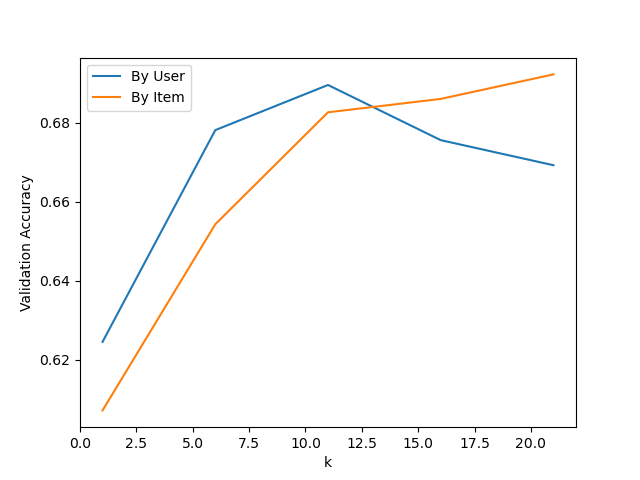
\includegraphics[width=0.85\textwidth]{final/knn.png}
        \caption{Validation accuracy with respect to $k$.}
        \label{fig:pAq1}
    \end{figure}
    \begin{table}[ht]
        \centering
        \begin{tabular}{|c|c|c|}
        \hline
        $k$ & \texttt{knn\_impute\_by\_user} & \texttt{knn\_impute\_by\_item} \\
        \hline
        1 & 0.624 & 0.607 \\
        6 & 0.678 & 0.654\\
        11 & \textbf{0.690} & 0.683 \\
        16 & 0.676 & 0.686 \\
        21 & 0.669 & \textbf{0.692} \\
        \hline
        \end{tabular}
    
        \caption{Data represented in Figure \ref{fig:pAq1}. Validation accuracy with respect to $k$ for distance by user and by item. The highest validation accuracies were obtained by $k^*=11$ and $k^*=21$ for user and input similarity respectively for which the test accuracies were $0.684$ and $0.682$ respectively.}
        \label{tab:pAq1}
    \end{table}

    \item \textbf{Item Response Theory}

    \begin{enumerate}[label = \textbf{\alph*}.]
        \item Given that
        $$
            z\eqdef p(c_{ij}=1\mid \theta_i,\beta_j)=\frac{\exp(\theta_i-\beta_j)}{1+\exp(\theta_i-\beta_j)},
        $$
        the (positive) log-likelihood $\log p(c_{ij}\mid \theta_i,\beta_j)$
        is given by:
        \begin{equation}
            \begin{aligned}
                \ell 
                &\eqdef \log p(c_{ij}\mid \theta_i,\beta_j) \\
                &= \log\!\Big( z^{c_{ij}}(1-z)^{1-c_{ij}} \Big) \\
                &= c_{ij}\log (z) + (1-c_{ij}) \log (1-z).
            \end{aligned}
            \label{irtll2}
        \end{equation}
        Using \eqref{irtll2}, we have
        $$
            \begin{aligned}
                \log p(\bf C\mid\bm\theta,\bm\beta)
                &= \log \prod_i \prod_j p(c_{ij}\mid \theta_i,\beta_j) \\
                &= \sum_i\sum_j \log p(c_{ij}\mid \theta_i,\beta_j) \\
                &= \sum_i\sum_j \ell = \sum_i\sum_j c_{ij}\log (z) + (1-c_{ij}) \log (1-z).
            \end{aligned}
        $$
        The partial derivatives of $\ell$ with respect to $\theta_i$ and $\beta_j$ are given by\footnote{Since $z$ is the sigmoid function, we have $\sfrac{\partial z}{\partial \theta_i}=z(1-z)$ and $\sfrac{\partial z}{\partial \beta_j}=-z(1-z)$.}
        $$
            \begin{aligned}
                \frac{\partial\ell}{\partial \theta_i}
                &= \frac{\partial\ell}{\partial z}\frac{\partial z}{\partial \theta_i} \\
                &= \left(\frac{c_{ij}}{z}-\frac{1-c_{ij}}{1-z}\right)z(1-z) \\
                &= c_{ij}(1-z)-z(1-c_{ij}) \\
                &= c_{ij}-c_{ij}z-z+c_{ij}z \\ 
                &= c_{ij}-z,
            \end{aligned}
            \quad \quad
            \begin{aligned}
                \frac{\partial\ell}{\partial \beta_j}
                &= \frac{\partial\ell}{\partial z}\frac{\partial z}{\partial \beta_j} \\
                &= \left(\frac{c_{ij}}{z}-\frac{1-c_{ij}}{1-z}\right)(-z(1-z)) \\
                &= \dots \\
                &= -c_{ij}+z.
            \end{aligned}
        $$

        \item The parameters $\bm \theta$ and $\bm \beta$ were randomly initialized element-wise using a uniform distribution over $[-0.1, 0.1]$ and optimized using the update rule\footnote{In each iteration, $\bm\theta$ is updated before $\bm\beta$.}
        $$
            \bm\theta \gets \bm\theta + \alpha\frac{\partial \ell}{\partial \bm\theta}\quad \bm\beta \gets \bm\beta + \alpha\frac{\partial \ell}{\partial \bm\beta}
        $$
        with learning rate $\alpha=0.001$ over 50 iterations.
        See Figures \ref{fig:pAq2b_1} and \ref{fig:pAq2b_2} for detailed results.
        \begin{figure}[h!]
            \centering
            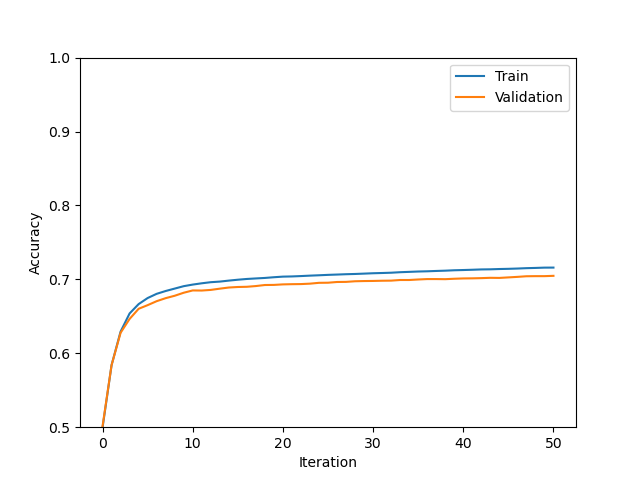
\includegraphics[width=.85\textwidth]{final/acc.png}
            \caption{Training and validation accuracy over time.}
            \label{fig:pAq2b_1}
        \end{figure}
        \begin{figure}[h!]
            \centering
            \begin{subfigure}[h!]{.46\textwidth}
                \centering
                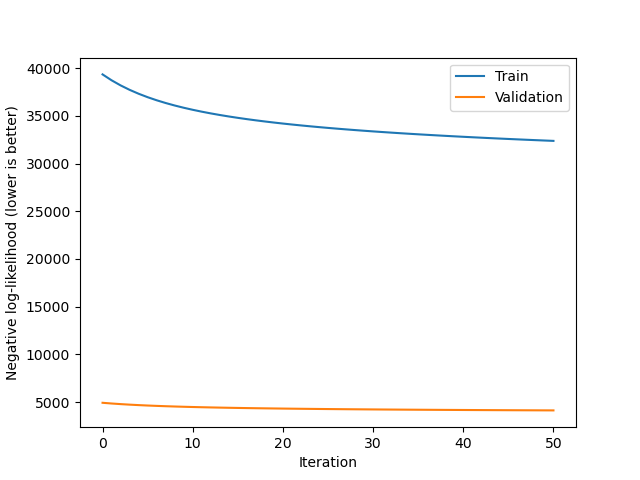
\includegraphics[width=.95\linewidth]{final/nll.png}
                \caption{Absolute negative log-likelihood. Note that the validation set, being significantly smaller, has a much smaller negative log-likelihood.}
            \end{subfigure}
            \quad
            \begin{subfigure}[h!]{.46\textwidth}
                \centering
                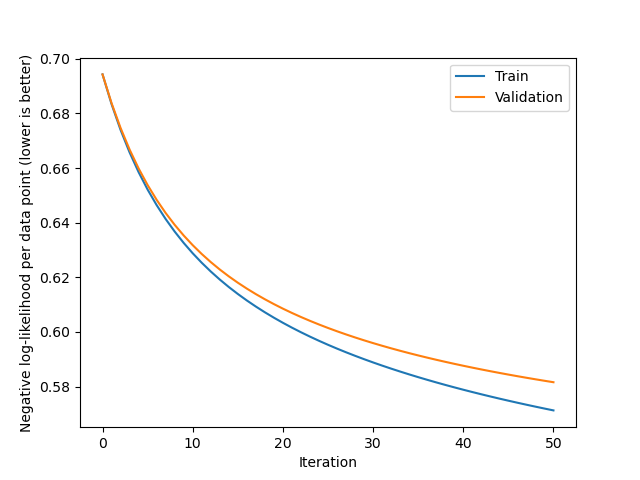
\includegraphics[width=.95\linewidth]{final/nll_norm.png}
                \caption{Negative log-likelihood, normalized by number of data-points.}
            \end{subfigure}
            \caption{Negative training and validation log-likelihood over time (lower is better).}
            \label{fig:pAq2b_2}
        \end{figure}

        \item The final training and validation accuracies after 50 iterations of training (see above) were 71.6\% and 70.3\% respectively\footnote{According to the Faculty of Arts and Science, this is equivalent to a B-}.

        \item See Figure \ref{fig:pAq2d}. Note the S-shape of the curve resulting from the use of the sigmoid function with respect to a linear variation over its parameter $\theta-\beta_j$. These plots may be interpreted as the predicted probability of success on a question with a measure of difficulty corresponding to $\beta_j$ with respect to student competency measured by $\theta$.

        \begin{figure}[h!]
            \centering
            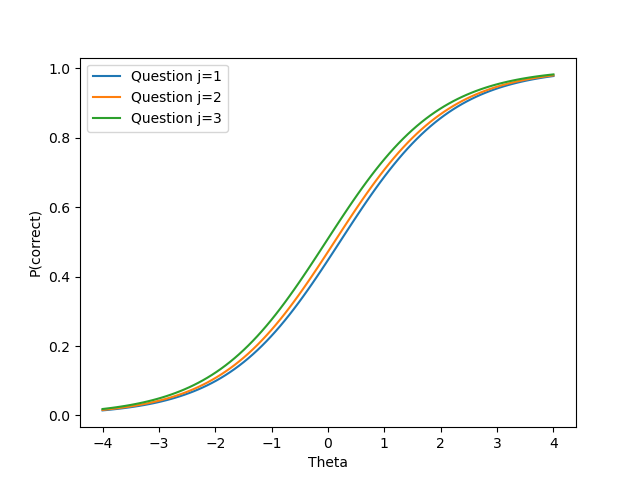
\includegraphics[width=.85\textwidth]{final/part_a_q2d.png}
            \caption{$p(\text{correct}\mid \theta,\beta_j)=\dfrac{\exp(\theta-\beta_j)}{1+\exp(\theta-\beta_j)}$ with respect to $\theta$ for $j\in\{1,2,3\}$.}
            \label{fig:pAq2d}
        \end{figure}
    \end{enumerate}

    \item \textbf{Option 2: Neural Networks}

    \begin{enumerate}[label = \textbf{\alph*}.]
        \item The differences between alternating least squares (ALS) and neural networks are as follows: 
        \begin{enumerate}
            \item Firstly, the purpose of ALS is to reduce the 
        high-dimensional input data into two lower-dimensional factor matrices meant to represent questions and students in the context of this problem. 
        Neural networks, on the other hand, attempt to represent the entirety of the data as a set of latent features rather than a differentiating between questions and students.
            \item Secondly, ALS alternates\footnote{Hence the name.} between optimizing each of the two latent feature matrices in order to
        factor the matrix, 
        while neural networks primarily use the multivariate chain rule to calculate the gradient in order to backpropagate, thus updating all of the weights of the network at once.
        
        \spacer
        
        ALS thus represents a more linear model optimized by an iterative process, whereas neural networks are nonlinear and more parallelizable.
            \item Thirdly, ALS is an unsupervised learning algorithm, 
        while neural networks can be used for both supervised and unsupervised learning. In this sense, the scope of neural networks 
        as a whole is much broader than that of ALS; neural networks can be used for a much wider set of tasks than simply dimensionality reduction.
        \end{enumerate}
        \item The forward pass was implemented according to the docstring.
        \item For every permutation of hyperparameters $(\alpha, n, k)$ of learning rate over
        $$
            \begin{aligned}
                \text{Learning rate}~~\alpha &\in \{0.01, 0.02, 0.03, 0.05, 0.1, 0.2, 0.3, 0.4, 0.5\} \\
                \text{Iteration count}~~n &\in \{10, 25, 50, 100\} \\
                \text{Model dimensionality}~~k &\in \{10,50,100,200,500\}
            \end{aligned}
        $$
        
        over iterations, $k^* = 50$ 
        was able to most consistently yield the highest validation accuracy. The highest validation accuracy with $k^* = 50$ was with a learning rate of $\alpha=0.01$ and $n=50$ iterations, yielding a validation accuracy of 68.1\%.
        \item The final test accuracy was 68.5\%. The training loss and validation accuracies over time are shown in Figure \ref{fig:pAq3d}. 

        \begin{figure}[h!]
            \centering
            \begin{subfigure}[h!]{.46\textwidth}
                \centering
                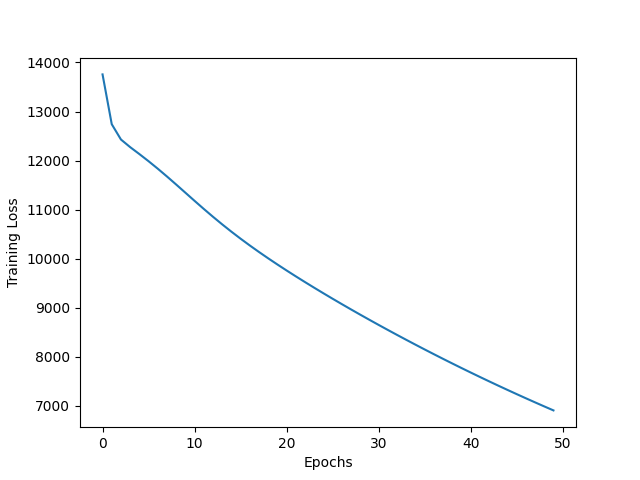
\includegraphics[width=.95\linewidth]{final/part_a_q3d1.png}
                \caption{Training loss over time without modified loss.}
            \end{subfigure}
            \quad
            \begin{subfigure}[h!]{.46\textwidth}
                \centering
                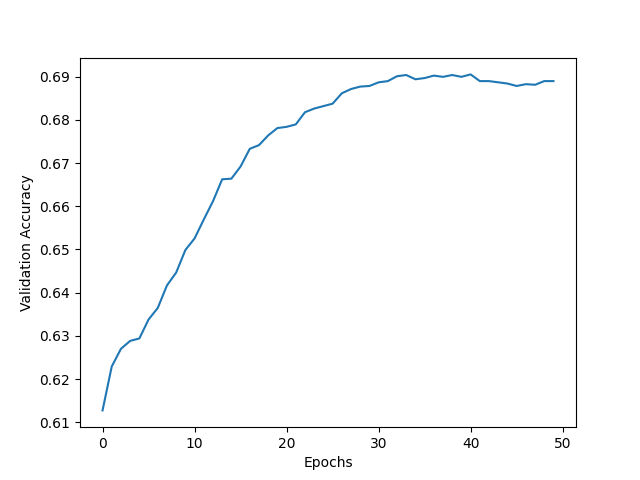
\includegraphics[width=.95\linewidth]{final/part_a_q3d2.png}
                \caption{Validation accuracy over time wihout modified loss.}
            \end{subfigure}
            \caption{Training loss and Validation accuracy over time without modified loss (lower loss and higher accuracy is better).}
            \label{fig:pAq3d}
        \end{figure}


        \item For the regularization term $\lambda = 0.001$, the 
        test accuracy was 68.4\%, 
        and the validation accuracy was 68.7\%.
        The adjusted loss function achieved a higher validation accuracy than the original loss function, 
        however, it had slightly lower test accuracy than the original test function. 
        The validation accuracy over time, as shown in \ref{fig:pAq3e}, behaves more erratically
        than when using the unmodified loss function, while the training loss over time behaves similarly to that of the unmodified loss function, though due to the added term, in the loss function, is shifted upwards.
        
        
        \begin{figure}[h!]
            \centering
            \begin{subfigure}[h!]{.46\textwidth}
                \centering
                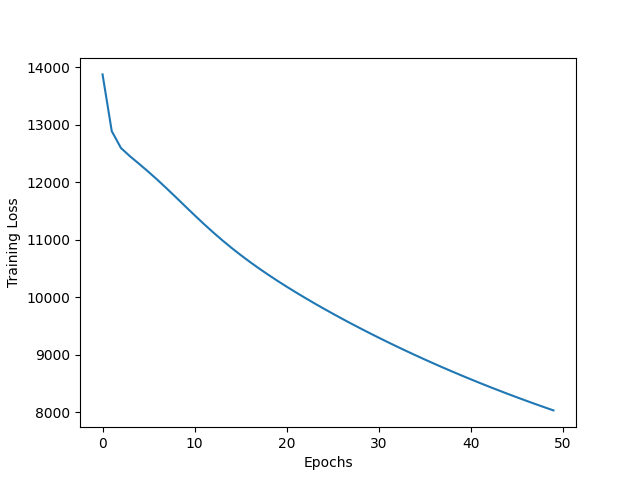
\includegraphics[width=.95\linewidth]{final/part_a_q3e1.png}
                \caption{Training loss over time with modified loss.}
            \end{subfigure}
            \quad
            \begin{subfigure}[h!]{.46\textwidth}
                \centering
                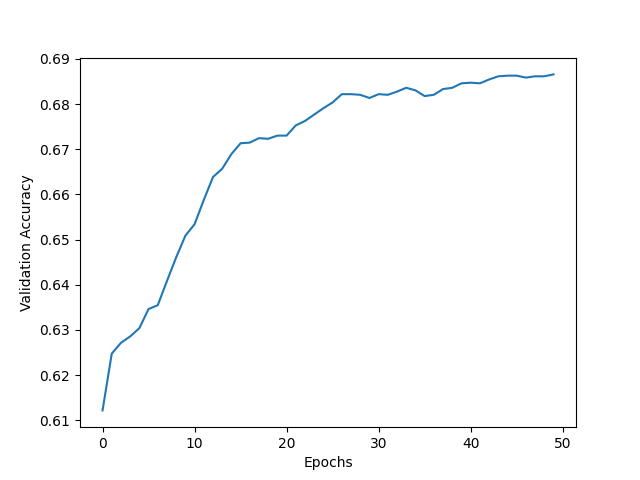
\includegraphics[width=.95\linewidth]{final/part_a_q3e2.png}
                \caption{Validation accuracy over time with modified loss.}
            \end{subfigure}
            \caption{Training loss and Validation accuracy over time with modified loss (lower loss and higher accuracy is better).}
            \label{fig:pAq3e}
        \end{figure}
    \end{enumerate}
\end{enumerate}

\newpage
\section*{Part B}

\subsection*{Introduction}

To attempt to improve on the results obtained in \textbf{Part A, Question 2–Item Response Theory}, we employ the use of a regularized \textit{multidimensional item response theory} (MIRT) model. Our underlying hypothesis is that the relatively low complexity of the original IRT model (and low resulting training accuracy providing evidence for underfitting) suggests that the performance of model may be improved in general by increasing the number of parameters.

\spacer

The model used is the one defined by \cite{mirt} and is a multidimensional generalization of the 2-parameter logistic (2PL) model, which is, in turn, a simplification of the 3-parameter logistic (3PL) first formulated by \cite{3pl}.

\subsection*{The MIRT Model}

A MIRT model with dimension $m$ predicts the probability of a given student $i$ answering a question $j$ as
$$
    p
    \eqdef p(c_{ij} = 1\mid \bm\alpha,\bm\theta,\bf d)
    = \frac{\exp(\bm\theta_{i}\cdot \bm\alpha_{j} + d_j)}{1+\exp(\bm\theta_{i}\cdot \bm\alpha_{j} + d_j)}
    = \frac{\displaystyle \exp\left(\sum_{\ell = 1}^m \theta_{i\ell}\alpha_{j\ell} + d_j\right)}{\displaystyle 
 1+\exp\left(\sum_{\ell = 1}^m \theta_{i\ell}\alpha_{j\ell} + d_j\right)}
$$

given parameters:

\begin{enumerate}
    \item $\bm\alpha$: a $N_{questions}\cross m$ matrix. By analogy to the original IRT model, the purpose of each row $\bm\alpha_\ell$ is comparable to that of $\bm\beta$ in the original model. In other words, in our MIRT model, each row is a latent representation of each question, whereas in our original model, each element of $\bm\beta$ is a scalar representation of each question (analogous to its difficulty).
    \item $\bm\theta$: a $N_{students}\cross m$ matrix. By analogy to the original IRT model, the purpose of each row $\bm\theta_\ell$ is comparable to that of $\bm\theta$ in the original model. In other words, in our MIRT model, each row is a latent representation of each student, whereas in our original model, each element of $\bm\theta$ is a scalar representation of each student (analogous to their competence).
    \item $\bf d$: a vector of size $N_{questions}$. Essentially a bias term (referred to as an ``intercept term" by \cite{mirt}).
\end{enumerate}

The dimension hyperparameter $m$ of the model is proportional to the complexity and number of parameters of the model. As will be discussed in more detail later, this value must be chosen carefully as to balance both the capability of the model to fit to the training data and the ability of the model to properly generalize.

\minisec{Model Optimization}

Similar to the original model, the log-likelihood function of the model is given by
$$
    \ell\eqdef \sum_{i}\sum_{j} c_{ij}\log (p) + (1 - c_{ij})\log(1-p).
$$
Optimization of this model is performed by iteratively applying the update rule
$$
    \bm\alpha \gets \bm\alpha + \gamma \frac{\partial \mathcal J}{\partial \bm \alpha} 
    \quad
    \bm\theta \gets \bm\theta + \gamma \frac{\partial \mathcal J}{\partial \bm \theta} 
    \quad
    \bf d \gets \bf d + \gamma \frac{\partial \mathcal J}{\partial \bf d}
$$
for a learning rate $\gamma$ and fitness function
$$
    \mathcal J = \ell - \lambda\mathcal R\footnote{Note that we subtract the regularization term from the log-likelihood term. Since we are looking to \textit{maximize} the log-likelihood, penalization should be done by \textit{subtracting} a quantity proportional to the complexity of the model.}
$$
where $\mathcal R = \norm{\bm \alpha}^2+\norm{\bm \theta}^2+\norm{\bf d}^2$ is an L2 regularization term used to prevent overfitting (this will be addressed in more detail later).

\subsection*{Model Visualization}

In the context of the original model, Figure \ref{fig:pAq2d} shows the resulting probability of correctness with respect to the parameter $\theta_i$ for some fixed $\beta_j$.
\spacer
In the context of the MIRT model, Figures \ref{fig:pB_3dplot1} and \ref{fig:pB_3dplot2} visualize the contour of $p(c_{ij} = 1\mid \bm\alpha_i,\bm\theta_i,\bf d)$ with respect to $\bm \theta_i\in\R^2$ for some fixed $\bm \alpha_j$. In some sense, $\bm \alpha_j$ acts as to linearly transform an $m$-dimensional sigmoid function $p$ in the space over $\bm\theta_j\in\R^m$, and vice versa. Intuitive interpretation of this visualization in the context of the student/question context is difficult, but these plots should be sufficient to demonstrate that the overall ``shape" of the model's output with respect to its parameters is only extended to higher dimensions rather than being fundamentally altered.

\begin{figure}[h!]
    \centering
    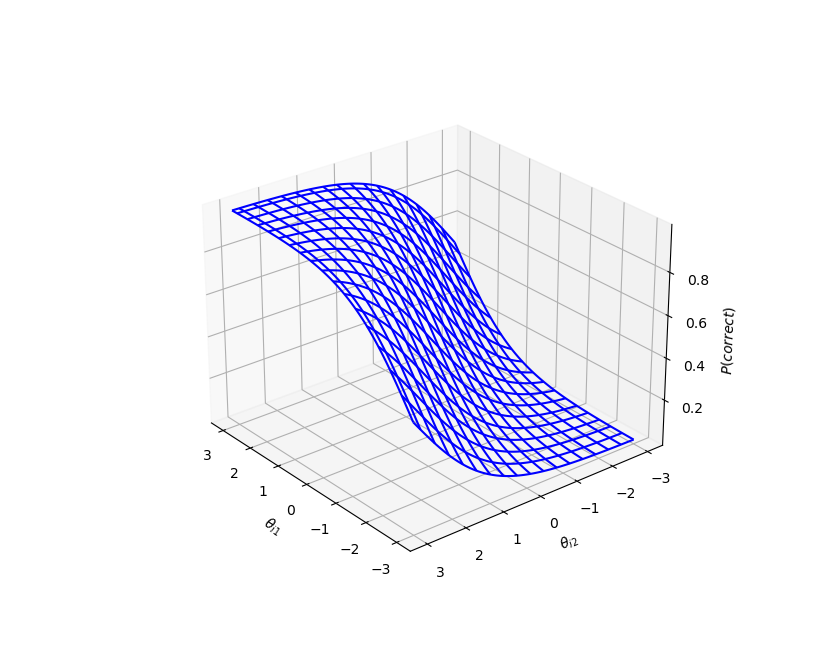
\includegraphics[width=0.85\textwidth]{final/3dplot.png}
    \caption{$p(c_{ij} = 1\mid \bm\alpha_j,\bm\theta_i,\bf d)$ with respect to $\bm \theta_i$. Note that $\bm\alpha$ has been fixed to $\langle 1, 1 \rangle$ for exemplary purposes.}
    \label{fig:pB_3dplot1}
\end{figure}

\begin{figure}[h!]
    \centering
    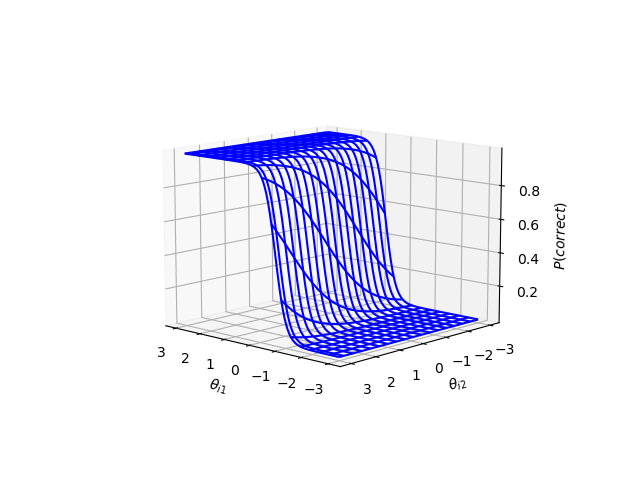
\includegraphics[width=0.85\textwidth]{final/3dplot_2.png}
    \caption{$p(c_{ij} = 1\mid \bm\alpha_j,\bm\theta_i,\bf d)$ with respect to $\bm \theta_i$. Note that $\bm\alpha$ has been fixed to $\langle 5, 1 \rangle$ for exemplary purposes.}
    \label{fig:pB_3dplot2}
\end{figure}

\newpage
\subsection*{Methodology}

We trained the model for 50 iterations with a learning rate $\gamma=0.02$. The model was initialized with dimensionality $m=3$ with a regularization weight $\lambda=2$. The hyperparameters $m$ and $\lambda$ were chosen via an automatic hyperparameter selection process wherein 100 pairs $(m,\lambda)$ were generated from a uniform distribution where
$$
    m\in\{2, 3,\dots,6\}\quad \lambda\in[0, 4],
$$
and the corresponding final validation accuracy $\mathcal A(m,\lambda)$ was evaluated after 50 training iterations as means of approximation for
$$
    \argmax_{(m,\lambda)} \mathcal A(m,\lambda).
$$

\subsection*{Results and Comparison}
Figure \ref{fig:pB_accplot1} shows the accuracy obtained by the model over time (i.e. with respect to number of iterations). The final validation accuracy was 69.7\%, and the final test accuracy was 69.6\%.

\spacer

\begin{figure}[h!]
    \centering
    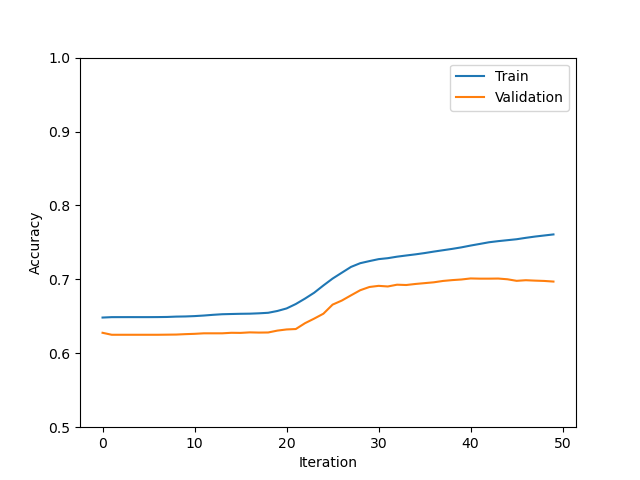
\includegraphics[width=0.85\textwidth]{final/partb_1.png}
    \caption{MIRT training and validation accuracy over time.}
    \label{fig:pB_accplot1}
\end{figure}

\begin{table}[h!]
    \centering
    \begin{tabular}{c|c|c}
        Model & Training Accuracy & Validation Accuracy \\
        \hline
        MIRT $(m=3, \lambda=2)$ & 76.1\% & 70.4\% \\
        MIRT $(m=3, \lambda=0)$ & 78.0\% & 69.4\% \\
        MIRT $(m=10, \lambda=0)$ & 88.6\% & 69.5\% \\
        IRT (original) & 71.6\% & 70.3\%
    \end{tabular}
    \caption{Results comparing the \textit{highest} (not final) training and validation accuracies obtained during training across different model configurations. MIRT $(m=3, \lambda=2)$ is the model configuration chosen for demonstration purposes.}
    \label{tab:pB_comp}
\end{table}

See Table \ref{tab:pB_comp}. Note the slightly lower resulting validation accuracy (and increased training accuracy) for the model configuration which omits the regularization term $(m=3,\lambda=0)$ when compared to the demonstration model. These results motivate the use of a regularization term to mitigate some of the effects of overfitting, likely from the increased model complexity. By taking this hypothesis to the extreme for the configuration $(m=10,\lambda=0)$, we see a dramatically improved training accuracy. While the \textit{highest} validation accuracy remains competitive with the other model configurations, Figure \ref{fig:pB_accplot2} shows as the model begins to improve with respect to its training accuracy, validation accuracy \textit{decreases} to 66.2\%, implying that the model has begun to overfit.

\subsection*{Model Limitations}

The results shown in Table \ref{tab:pB_comp} implies that the MIRT model, with its arbitrary complexity and capability of fitting to the training data, is still limited in its ability to generalize. Although further analysis is warranted, we propose two immediate hypotheses:

\begin{enumerate}
    \item The model's learned latent representations $\bm \alpha$ and $\bm \theta$ of information about the questions and students lack in generalizability. In other words, these parameter vectors encode too much information about the training data points themselves rather than providing a general representation of their corresponding subjects.

    \spacer
    
    This problem may potentially be addressed by changing the regularization metric used; the L2 regularization metric used for the purposes of demonstration is a fairly naïve metric, and problem-specific information could be applied to optimize the regularization method further.
    \item The increased number of parameters in the model necessitates more training data. In other words, the ratio of training data points to $N_{students}\cross N_{items}$ is too small for the purposes of sufficiently training this model. A case for this hypothesis is made by considering the much smaller difference between the training and validation accuracies of the smaller, original IRT model.

    \spacer

    While the amount of training data provided is non-negotiable, this hypothesis may be tested by artificially omitting training data to see the resulting impact on validation accuracy. In other words, given a model $\bf M$ (i.e. the MIRT model or the original IRT model), we may define a function
    $$
        \mathcal A(p\mid \bf M)
    $$
    describing the resulting training accuracy as a function of a proportion $0\leq p\leq 1$ limiting the amount of original training data for the purposes of training.
    
    \spacer
    
    If we see that as $p$ approaches 1, we do not see a significant improvement in $\mathcal A$, then by extrapolation\footnote{Specifically, we would attempt to use this data to predict $\mathcal A(p)$ as $p$ increases beyond 1 to determine whether the model might benefit from additional training data, if it were somehow obtained.}, we may assume that the model $\bf M$ is not limited by the amount of training data provided, rather, the model is being limited by some other factor inherent to the model itself (see hypothesis 1). 
\end{enumerate}

\subsection*{Conclusions}

As shown in Table \ref{tab:pB_comp}, we see that the MIRT model is essentially equivalent to the original model in terms of validation accuracy. Despite this, the pattern of consistently higher training accuracies for the MIRT model when compared to the original model supports the original hypothesis that model complexity (specifically the model's dimesnion $m$) is proportional to the model's capability to fit the training data.

\spacer

With respect to the data given, the modifications to this model do not provide clear improvements when evaluated over the datasets on which the model was not directly trained. Despite this, both the flexible complexity of the model and demonstrably improved capability of fitting to the training data provide a compelling case for MIRT as a more robust model compared to the original model in applications where a greater relative quantity of training data is available. 

\begin{figure}[H]
    \centering
    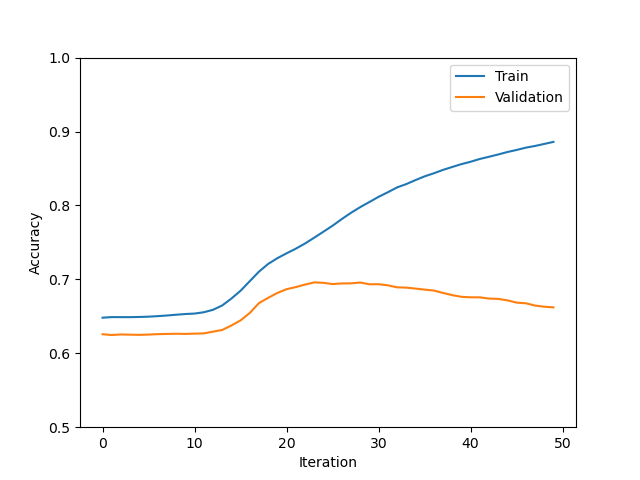
\includegraphics[width=0.85\textwidth]{final/partb_2.png}
    \caption{MIRT training and validation accuracy over time for $(m=10,\lambda=0)$, an extreme example of high model dimensionality demonstrating the capability of the model to better fit the provided data, generalizability notwithstanding.}
    \label{fig:pB_accplot2}
\end{figure}

\section*{Individual Contributions}

The work on this project was distributed between its authors as follows:

\begin{itemize}
    \item \textbf{Ian Huang}
        \begin{itemize}
            \item Typesetting and editing.
            \item Part A, Question 1 and 2.
            \item Part B: research and analysis.
        \end{itemize}
    \item \textbf{Benjamin Liu}
        \begin{itemize}
            \item Part A, Questions 3 and 4.
            \item Part B: hyperparameter tuning, data visualization.
            \item Derivations, gradient checking.
        \end{itemize}
\end{itemize}

\newpage

\bibliography{final}

\end{document}